%!TEX root = ../aberdeen21.tex

\begin{frame}[t]{Beyond the even prime}

	\pause

	Extending the diagonal to a full \textcolor{pblue}{$E_\infty$-coalgebra} structure on chains.

	\smallskip\pause

	These provide an algebraic model for the homotopy theory of spaces.\\ e.g. over $\mathbb Q$ (Quillen--Sullivan) over $\overline{\mathbb F}_p$ (Mandell).

	\smallskip\pause

	\begin{theorem}[Med.]
		The collection of maps $\gchains(\gsimplex^n) \to \gchains(\gsimplex^n)^{\otimes r}$ obtained from compositions of
		\begin{align*}
		\Delta &\colon \gchains(\gsimplex^n) \to \gchains(\gsimplex^n)^{\otimes 2}
		\qquad \text{(AW diagonal)} \\
		\ast &\colon \gchains(\gsimplex^n)^{\otimes 2} \to \gchains(\gsimplex^n)
		\qquad \text{(Join map)}
		\end{align*}
		defines an $E_\infty$-coalgebra on simplicial chains.
	\end{theorem}

	\pause \only<5>{\qquad \qquad \scalebox{0.7}{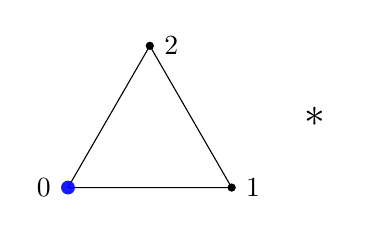
\begin{tikzpicture}[scale=.6]
\coordinate (A) at (210:2);
\coordinate (B) at (-30:2);
\coordinate (C) at (90:2);

\draw[draw=black] (A) -- (B) -- (C) -- (A);

\node[circle,fill=blue, opacity=.9, inner sep=0pt,minimum size=5pt, label=left:{0}] (a) at (A) {};
\node[circle,fill=black,inner sep=0pt,minimum size=3pt, label=right:{$1$}] (a) at (B) {};
\node[circle,fill=black,inner sep=0pt,minimum size=3pt, label=right:{$2$}] (a) at (C) {};

\node[scale=1.5] at (3.5,0.5) {$\ast$};
\end{tikzpicture}
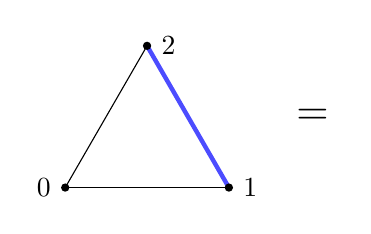
\begin{tikzpicture}[scale=.6]
\coordinate (A) at (210:2);
\coordinate (B) at (-30:2);
\coordinate (C) at (90:2);

\draw[draw=blue,  ultra thick, draw opacity=.7] (B) -- (C);
\draw[draw=black] (C) -- (A);
\draw[draw=black] (A) -- (B);

\node[circle,fill=black,inner sep=0pt,minimum size=3pt, label=left:{$0$}] (a) at (A) {};
\node[circle,fill=black,inner sep=0pt,minimum size=3pt, label=right:{$1$}] (a) at (B) {};
\node[circle,fill=black,inner sep=0pt,minimum size=3pt, label=right:{$2$}] (a) at (C) {};

\node[scale=1.5] at (3.5,.5) {=};
\end{tikzpicture}
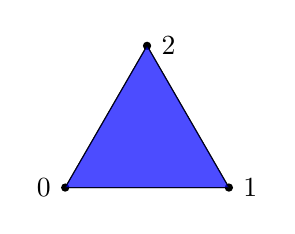
\begin{tikzpicture}[scale=.6]
\coordinate (A) at (210:2);
\coordinate (B) at (-30:2);
\coordinate (C) at (90:2);

\draw[draw=black] (A) -- (B) -- (C) -- (A);

\node[circle,fill=black,inner sep=0pt,minimum size=3pt, label=left:{$0$}] (a) at (A) {};
\node[circle,fill=black,inner sep=0pt,minimum size=3pt, label=right:{$1$}] (a) at (B) {};
\node[circle,fill=black,inner sep=0pt,minimum size=3pt, label=right:{$2$}] (a) at (C) {};

\draw[draw, fill=blue, opacity=.7] (A) -- (B) -- (C) -- (A);
\end{tikzpicture}}} \pause

	Used to introduce cup $(p,i)$-products effectively def. \textcolor{pblue}{Steenrod operations} on mod $p$ cohomology.
	\pause (Implemented in \texttt{comch}, a project I develop.)

	\smallskip\pause

	\only<8>{Also, versions for: \textcolor{pblue}{cubical} (R. Kaufmann) and
	\textcolor{pblue}{multisimplicial} chains (A. Pizzi \& P. Salvatore).}
\end{frame}

\begin{frame}{Other math I would be happy to discuss with you}
	\begin{itemize}
		\item \pause Higher category theory
		\item \pause Representation \& cohomology of small categories
		\item \pause Algebraic surgery theory
		\item \pause Geometric cohomology
		\item \pause Functional topology \& persistence theory
		\item \pause Higher information theory \& hyperharmonic analysis
		\item \pause Adams'/Baues' cobar \& string topology
		\item \pause Khovanov homology
		\item \pause Fiber polytopes
		\item \pause Frobenius algebras \& TQFTs
		\item \pause $E_n$-operads \& Dyer-Lashoff-Cohen operations
		\item \pause $C_\infty$-coalgebras \& rational homotopy theory
		\item \pause $A_\infty$-algebras \& symplectic geometry
		\item \dots
	\end{itemize}
\end{frame}
